\PassOptionsToPackage{hyperfootnotes=false}{hyperref}
\documentclass[a4paper,fleqn]{cas-sc}
\usepackage[pagewise]{lineno}
% \linenumbers

\usepackage[numbers]{natbib}
\usepackage[version=4]{mhchem}
\usepackage{cleveref}
\usepackage{subcaption}
\usepackage{longtable}
\usepackage{mathtools}
\usepackage{tabularx}
\usepackage{makecell}
\usepackage{booktabs}
\usepackage{adjustbox}
\usepackage{xspace}
\renewcommand\cellalign{tl}
\newcolumntype{P}[1]{>{\centering\arraybackslash}p{#1}}
\usepackage{xcolor}
\usepackage{siunitx}
\usepackage{xurl}
\graphicspath{{figures/generated/}}

\newcommand{\Ha}{\text{Ha}}
\newcommand{\COtwo}{\ce{CO2}\xspace}
\newcommand{\HtwoO}{\ce{H2O}\xspace}
\newcommand{\MEA}{\ce{MEA}\xspace}
\newcommand{\MEAH}{\ce{MEAH+}\xspace}
\newcommand{\MEACOO}{\ce{MEACOO-}\xspace}
\newcommand{\HCOthree}{\ce{HCO3-}\xspace}
\newcommand{\COthree}{\ce{CO3^2-}\xspace}
\newcommand{\HthreeO}{\ce{H3O+}\xspace}
\newcommand{\Hydroxide}{\ce{OH-}\xspace}
\newcommand{\Ntwo}{\ce{N2}\xspace}
\newcommand{\Otwo}{\ce{O2}\xspace}
\newcommand{\NtwoO}{\ce{N2O}\xspace}

\newcommand{\A}{\text{A}}
\newcommand{\B}{\text{B}}
\newcommand{\C}{\text{C}}
\newcommand{\D}{\text{D}}
\newcommand{\code}[1]{\texttt{#1}}
\newcommand{\liq}{\ell}
\newcommand{\vap}{v}

\begin{document}

\let\WriteBookmarks\relax
\def\floatpagepagefraction{1}
\def\textpagefraction{.001}

\shorttitle{ePC-SAFT with carbamate chemistry for CO2 in aqueous MEA}
\shortauthors{Polley}

\title[mode = title]{\texorpdfstring{Electrolyte PC-SAFT with carbamate chemistry for \ce{CO2} in aqueous monoethanolamine: the role of the Born term and of speciation data}{Electrolyte PC-SAFT with carbamate chemistry for CO2 in aqueous monoethanolamine: the role of the Born term and of speciation data}}

\author[1]{Tanner W. Polley}[orcid=0009-0008-5957-4152]
\cormark[1]
\ead{tpolley3@byu.edu}

\affiliation[1]{
    organization={Department of Chemical Engineering, Brigham Young University},
    city={Provo},
    state={UT},
    postcode={84602},
    country={United States}
}

\cortext[cor1]{Corresponding author.}

\begin{abstract}
% P:abstract-01
The equilibrium \COtwo partial pressure over loaded aqueous monoethanolamine (\MEA) depends on liquid speciation, and titration and NMR measurements disagree on bicarbonate.
Electrolyte PC-SAFT (ePC-SAFT) with explicit ions has been applied to aqueous methyldiethanolamine, which forms no carbamate, and recent Born-term modifications were parameterized on salt solutions.
We fit five interaction coordinates of a nine-species ePC-SAFT model with explicit carbamate chemistry to 48 \COtwo partial pressures (40 and \SI{60}{\degreeCelsius}) and 94 species targets (20--\SI{60}{\degreeCelsius}) in 30 wt\% \MEA, with average absolute relative deviations (AARD) of 13.53\,\% and 8.28\,\%.
The ranking of the solvation-shell and dielectric-saturation (SSM+DS) and Original Born terms depends on the role of 18 titration bicarbonate observations and on inherited Born inputs: with interactions fixed, Original Born reaches a cost of 32.18 against 32.99 for SSM+DS at 0.8 times three ion Born diameters or an \MEA permittivity of 24.
The Born term itself matters: refitting without it raises the cost to 98.79, and fixing the \MEAH--\MEACOO or \MEAH--water interaction at zero raises it by 134.3 or 75.9.
Outside the present fit, the pressure AARD is 20.27\,\% for 21 rows at \SI{80}{\degreeCelsius}, whose data informed fixed inputs, and 24.51\,\% for 11 previously unused rows near \SI{353}{\kelvin}; refitting with source reaction constants to data at or below \SI{60}{\degreeCelsius} gives 29.33 and 52.30\,\%, so independent temperature information is required.
The bicarbonate--water coefficient lies at its bound, density and heat capacity are not qualified, and no physical validation is claimed.
\end{abstract}

\begin{keywords}
\COtwo solubility\sep{}ePC-SAFT\sep{}modified Born term\sep{}monoethanolamine\sep{}chemical speciation\sep{}reactive vapor--liquid equilibrium
\end{keywords}

\maketitle

\hypersetup{
    pdftitle={Electrolyte PC-SAFT with carbamate chemistry for CO2 in aqueous monoethanolamine: the role of the Born term and of speciation data},
    pdfauthor={Tanner W. Polley},
    pdfsubject={Born-term choice and speciation-data role in a nine-species ePC-SAFT model of CO2 in 30 wt\% aqueous MEA},
    pdfkeywords={carbon dioxide, monoethanolamine, ePC-SAFT, modified Born term, speciation, vapor-liquid equilibrium}
}

\section{Introduction}\label{sec:introduction}
% P:introduction-01
Monoethanolamine (\MEA) in water is the reference solvent for \COtwo absorption, and its vapor--liquid equilibrium has been measured extensively~\cite{Jou1995,Mamun2005,Hilliard2008,Aronu2011,Xu2011}.
Absorbed \COtwo reacts with water and amine to form protonated amine, carbamate, bicarbonate and carbonate.
The equilibrium \COtwo partial pressure at a given loading therefore depends on both the phase equilibrium and the liquid speciation.
A model can reproduce the pressure with an implausible distribution of \MEA, \MEAH, \MEACOO, \HCOthree and \COthree, so speciation measurements provide a separate test of the same thermodynamic state.

% P:introduction-02
Speciation measurements for loaded \MEA differ in what they observe.
Quantitative NMR resolves carbamate and bicarbonate, but fast proton exchange permits only the sum of \MEA and \MEAH to be observed~\cite{Bottinger2008,Jakobsen2005}.
Matin et al.\ obtained all four major species from acid and base titrations combined with a total carbon measurement~\cite{matinFacileMethodDetermination2012}.
They reported agreement with NMR for free amine, protonated amine and carbamate, and bicarbonate higher than the NMR values~\cite[pp.~6616--6617]{matinFacileMethodDetermination2012}.
When such observations enter a parameter fit, the choice of which measurements to fit can affect which model form is selected.

% P:introduction-03
Excess-Gibbs-energy models with chemical equilibria represent this system with fitted interaction parameters.
B\"ottinger et al.\ refitted the \MEA carbamate-formation constant to NMR speciation while retaining the Bates--Pinching protonation constant and published \MEA interaction parameters~\cite{Bottinger2008}.
Akula et al.\ fitted an electrolyte NRTL model jointly to \COtwo pressure and heat of absorption, leaving NMR speciation and heat capacity outside the fit~\cite{Akula2023a}.
Equations of state based on statistical associating fluid theory describe association and chain formation within one Helmholtz energy~\cite{Gross2001,Gross2002}.
PC-SAFT and SAFT-HR have been applied to loaded \MEA with a separate chemical-equilibrium calculation and neutral-species fugacities~\cite{Baygi2015,Najafloo2018}.

% P:introduction-04
Electrolyte PC-SAFT (ePC-SAFT) adds a Debye--H\"uckel contribution for charged species~\cite{Cameretti2005}, and Held et al.\ estimated ion parameters from densities and osmotic coefficients of aqueous salt solutions, with dispersion between ions of the same sign excluded~\cite{Held2014}.
Uyan et al.\ and Wangler et al.\ applied ePC-SAFT with explicit ions and activity-coupled reaction equilibria to aqueous MDEA, and predicted acid-gas solubility from parameters obtained from pure components and binary subsystems~\cite{Uyan2015,Wangler2018}.
Later work added concentration-dependent permittivity to the Born and Debye--H\"uckel terms~\cite{Bulow2020,Rueben2024} and predicted \COtwo solubility in aqueous and organic salt solutions~\cite{Schick2023}.
Figiel et al.\ modified the Born term to account for the solvation-shell volume and dielectric saturation near an ion (SSM+DS), with parameters estimated from ion solvation and salt activity data in water and alcohols at \SI{298.15}{\kelvin}~\cite{Figiel2025}; a later correction restored a missing bracket and the ion-region permittivity in its Eq.~(7)~\cite{Figiel2026Correction}.
Carbamate-forming \MEA differs from these test systems because the ion population and the solvent composition change together with \COtwo loading through reaction equilibrium.

% P:introduction-05
This work fits a nine-species ePC-SAFT model with explicit carbamate chemistry to \COtwo partial pressure in 30 wt\% \MEA at 40 and \SI{60}{\degreeCelsius} and to speciation at 20--\SI{60}{\degreeCelsius}.
Its parameters are fitted to ternary \MEA--\COtwo--\HtwoO pressure and speciation data.
In the MDEA studies above, prediction means calculation of a mixture with no parameter adjusted to that mixture~\cite{Uyan2015,Wangler2018}.
That meaning does not apply here, so calculations at conditions outside the present fit are reported as tests outside the fit; above \SI{60}{\degreeCelsius} and at other amine concentrations, they are extrapolations.
\Cref{tab:literature-model-comparison} summarizes the quantities fitted and left outside the fit in this and the closest published studies.

\begin{table*}[pos=!tb,width=\textwidth]
    \centering
    \footnotesize
    \caption{Fitted and outside-fit quantities in published models closest to the present model and in this work.
    ``Outside fit'' refers to quantities excluded from the parameter-estimation step described in each row.
    For the present work, it refers only to the five-parameter fit to 149 targets; the fixed reaction shifts and \COtwo dispersion energy were estimated using data that included \SI{80}{\degreeCelsius}.}
    \label{tab:literature-model-comparison}
    \begin{tabularx}{\textwidth}{@{}>{\raggedright\arraybackslash}p{2.4cm}>{\raggedright\arraybackslash}p{3.2cm}>{\raggedright\arraybackslash}X>{\raggedright\arraybackslash}X@{}}
        \toprule
        Study & System and model & Quantities used for fitting & Quantities outside the fit \\
        \midrule
        B\"ottinger et al.~\cite{Bottinger2008} & \MEA--\HtwoO--\COtwo; extended Pitzer excess Gibbs energy with chemical equilibria & \MEA carbamate-formation and oxazolidone-formation constants fitted to NMR; \MEA protonation constant and \MEA interaction parameters retained from the literature (\S\S5--6) & Vapor--liquid equilibrium (\S6) \\
        Baygi and Pahlavanzadeh~\cite{Baygi2015} & \MEA--\HtwoO--\COtwo; PC-SAFT with separate chemical-equilibrium calculation & \MEA pure-component parameters; binary interaction parameters from binary vapor--liquid equilibrium & Ternary \COtwo solubility \\
        Najafloo and Zarei~\cite{Najafloo2018} & \MEA--\HtwoO--\COtwo; SAFT-HR & Pure-\MEA vapor pressure and liquid density (\S3.1); literature \COtwo--\HtwoO interaction and zero \COtwo--\MEA and \MEA--\HtwoO interactions (\S3.2) & Ternary solubility comparisons (\S3.3); the conclusion describes the data use more broadly than the parameter-estimation methods \\
        Chremos et al.~\cite{chremosModellingPhaseChemical2016} & \MEA--\HtwoO--\COtwo; SAFT-$\gamma$ square well with association-derived species & Group parameters from pure and mixture data; reactive interactions from 30 wt\% \MEA solubility at \SI{353.15}{\kelvin} (\S3.6) & Carbamate and bicarbonate speciation; temperature and amine transfer \\
        Perdomo et al.~\cite{perdomoPredictiveGroupcontributionFramework2023} & Aqueous amines--\COtwo; SAFT-$\gamma$ Mie with association-derived species & Group interactions from pure and mixture properties; primary alkanolamine--\COtwo interactions from 30 wt\% \MEA VLE at 298.15 and \SI{313.15}{\kelvin} (\S4.3.3) & \MEA/DEA speciation; higher-temperature VLE \\
        Lloret et al.~\cite{lloretConsistentTransferableThermodynamic2017} & \MEA--\HtwoO--\COtwo; soft-SAFT with reactive association & Molecular and cross-association parameters from pure/binary data; reactive \COtwo association sites from ternary VLE (\S4.7) & Transfer to another \MEA concentration \\
        Akula et al.~\cite{Akula2023a} & \MEA--\HtwoO--\COtwo; electrolyte NRTL & \COtwo partial pressure and heat of absorption, jointly (Eq.~34) & NMR speciation and liquid heat capacity (\S4.2) \\
        Uyan et al.~\cite{Uyan2015} & MDEA--\HtwoO--\COtwo; ePC-SAFT with explicit ions & Literature pure-component and ion parameters; binary parameters from binary subsystems & Ternary \COtwo solubility \\
        Wangler et al.~\cite{Wangler2018} & MDEA--\HtwoO--\COtwo/\ce{H2S}; ePC-SAFT with explicit ions & Binary parameters including osmotic coefficients of water--MDEA--HCl & \COtwo and \ce{H2S} solubility; enthalpy of absorption \\
        Figiel et al.~\cite{Figiel2025} & Salts in water, methanol and ethanol; ePC-SAFT with SSM+DS Born term & Born diameters to infinite-dilution solvation Gibbs energies in water; solvent factors to NaBr activity coefficients; aqueous ion interactions to salt activity or osmotic data; ion--methanol and ion--ethanol interactions to infinite-dilution solvation Gibbs energies; \SI{298.15}{\kelvin} & Transfer Gibbs energies and activity coefficients in mixed solvents \\
        This work & 30 wt\% \MEA--\HtwoO--\COtwo; nine-species ePC-SAFT, SSM+DS or original Born & Five binary interaction parameters to 47 \COtwo pressures at 40/\SI{60}{\degreeCelsius}, 94 species at 20/40/\SI{60}{\degreeCelsius} and eight integral heats at \SI{40}{\degreeCelsius} & \COtwo pressure and species at \SI{80}{\degreeCelsius}; pressures near 353 and \SI{392}{\kelvin}; 100--\SI{120}{\degreeCelsius}; 15 and 45 wt\% \MEA; Arcis integral heats at \SI{322.5}{\kelvin} \\
        \bottomrule
    \end{tabularx}
\end{table*}


% P:introduction-06
The work makes three contributions.
First, it compares the SSM+DS and Original Born terms in \MEA with identical fitted coordinates and data, and shows that their ranking depends on the role assigned to the bicarbonate observations of Matin et al., which those authors report as higher than NMR values, and on inherited Born inputs; it does not establish which measurement method or Born form is more accurate.
Second, it measures how the fitted response depends on fixed Born inputs and on each interaction coordinate, through fixed-interaction scans, refits with one coordinate fixed at zero and a refit without the Born term.
These show that the Born term itself is needed, that the \MEAH--\MEACOO and \MEAH--water interactions carry most of the fit, and that the interactions compensate locally for small changes in five specified Born inputs at the historical optimum but not for removal of the Born term.
Third, it tests the record outside the present fit, at 80 and 100--\SI{120}{\degreeCelsius}, including measurements not used at any earlier stage, and at 15 and 45 wt\% \MEA; a refit restricted to data at or below \SI{60}{\degreeCelsius} shows that these data do not determine the temperature response.
It also states the limits of the record: an interaction coefficient at its bound, the carbonate partition, density and heat capacity.
No physical validation of the model at new conditions is claimed.

\section{Thermodynamic model}\label{sec:theory}
% P:theory-01
The liquid contains nine true species: \COtwo, \MEA, \HtwoO, \MEAH, \MEACOO, \HCOthree, \COthree, \HthreeO and \Hydroxide.
Each equilibrium state is a reactive bubble state of one liquid and one incipient vapor at the measured temperature and apparent composition.
Only the neutral species \COtwo, \MEA and \HtwoO enter the vapor, and the calculated \COtwo partial pressure is \(p_{\COtwo}=y_{\COtwo}P\).
The same ePC-SAFT equation of state describes both phases.

\subsection{Residual Helmholtz energy}
% P:theory-02
The reduced residual Helmholtz energy is the sum of hard-chain, dispersion, association, Debye--H\"uckel and Born contributions \cite{Gross2001,Gross2002,Cameretti2005,Held2014,Figiel2025}:
\begin{equation}
    a^{\mathrm{res}}
    =
    a^{\mathrm{hc}}
    +a^{\mathrm{disp}}
    +a^{\mathrm{assoc}}
    +a^{\mathrm{DH}}
    +a^{\mathrm{Born}} .
    \label{eq:epcsaft-residual-split}
\end{equation}
The hard-chain and dispersion terms follow Gross and Sadowski \cite{Gross2001}, with the dispersion energy of a pair given by
\begin{equation}
    u_{ij}=\sqrt{u_iu_j}\,\left(1-k_{ij}\right).
    \label{eq:dispersion-combining-rule}
\end{equation}
Dispersion between ions of the same charge sign, including an ion with itself, is excluded, while ion--solvent and cation--anion pairs keep \cref{eq:dispersion-combining-rule} \cite{Figiel2025}.
The \MEAH--water interaction depends on temperature,
\begin{equation}
    k_{\MEAH,\HtwoO}(T)=k_{\MEAH,\HtwoO}+b\left(\frac{1}{T}-\frac{1}{T_{\mathrm{ref}}}\right),
    \qquad T_{\mathrm{ref}}=\SI{313.15}{\kelvin},
    \label{eq:kij-temperature}
\end{equation}
and every other \(k_{ij}\) is constant.
Ion hard-chain and Debye--H\"uckel diameters are \(d_i=0.88\,\sigma_i\) \cite[Eq.~4]{Figiel2025}.

% P:theory-03
Water and \MEA carry two association sites (2B), and \COtwo carries two induced-association sites that bond only with water \cite{Kleiner2007,Pabsch2020,Schick2023}.
The \COtwo--water cross-association energy is \SI{1212.85}{\kelvin}, half the water self-association energy, with the water association volume \cite[Table~1, Sect.~2.4.2]{Schick2023}.
\MEA--water cross-association follows the Wolbach--Sandler rule used by Fakouri Baygi and Pahlavanzadeh \cite[Eq.~6]{Baygi2015}.
The association strength carries \(\sigma_{ij}^3\), so their \MEA association volume, reported for a \(d_{ij}^3\) strength \cite[Table~2]{Baygi2015}, was converted from 0.037470 to 0.036287, the constant value that best reproduces the vapor pressure and saturated-liquid density of their model at 293.15--\SI{393.15}{\kelvin}.

\subsection{Born contribution with solvation shell and dielectric saturation}
% P:theory-04
The Born term follows the solvation-shell and dielectric-saturation (SSM+DS) form of Figiel et al.\ \cite[Eqs.~5--10]{Figiel2025}, with its Eq.~7 as corrected in 2026 \cite{Figiel2026Correction}:
\begin{equation}
    a^{\mathrm{Born}}
    =
    -\frac{e^2}{4\pi\varepsilon_0k_{\mathrm{B}}T}
    \sum_{i\in\mathcal{I}}x_iz_i^2
    \left[
        \frac{1-\varepsilon_{\mathrm{bulk}}^{-1}}{D_i}
        +c_{\mathrm{dielectric}}\left(1-\varepsilon_{\mathrm{ion}}^{-1}\right)
        \left(\frac{1}{d_i^{\mathrm{Born}}}-\frac{1}{D_i}\right)
    \right],
    \label{eq:born-ssm-ds}
\end{equation}
\begin{equation}
    D_i=d_i^{\mathrm{Born}}\left[1+c_{\mathrm{shell}}\frac{f_{\mathrm{mix}}-1}{|z_i|}\right],
    \qquad
    f_{\mathrm{mix}}=\frac{\sum_kx_kf_k}{\sum_kx_k}.
    \label{eq:born-shell-diameter}
\end{equation}
Here \(\mathcal{I}\) is the set of ions, \(d_i^{\mathrm{Born}}\) is the Born diameter, \(D_i\) is the outer diameter of the first solvation shell and \(\varepsilon_{\mathrm{ion}}=8\) is the permittivity assigned to the region between the ion surface and that shell.
The selected model uses \(c_{\mathrm{shell}}=c_{\mathrm{dielectric}}=1\), which reproduces the corrected Eq.~7; the original Born comparison uses \(c_{\mathrm{shell}}=c_{\mathrm{dielectric}}=0\), which recovers the original Born expression \cite[Eq.~5]{Figiel2025}.
The water solvation factor is \(f_{\HtwoO}=1.5\) \cite[Table~2]{Figiel2025}, and every other component, including \MEA, \COtwo and all ions, has \(f_k=1\).
Figiel et al.\ restrict the average in \cref{eq:born-shell-diameter} to ions and solvents; here it runs over all nine components, so \(f_{\mathrm{mix}}=1+0.5\,x_{\HtwoO}\).
The shell diameter therefore changes with loading through the water mole fraction, and the Born term contributes to the water activity.

\subsection{Relative permittivity}
% P:theory-05
The bulk permittivity in the Debye--H\"uckel and Born terms is the mass-weighted permittivity of the neutral solvents,
\begin{equation}
    \varepsilon_{\mathrm{bulk}}
    =
    \frac{\sum_{s\in\mathcal{S}}x_sM_s\varepsilon_s}{\sum_{s\in\mathcal{S}}x_sM_s},
    \qquad \mathcal{S}=\{\HtwoO,\MEA\},
    \label{eq:solvent-permittivity}
\end{equation}
which is the salt-free weight-fraction rule of Uyan et al.\ and Figiel et al.\ \cite[Eq.~5]{Uyan2015}\cite[Eq.~12]{Figiel2025}.
The ion-fraction suppression of Figiel et al.\ \cite[Eq.~11]{Figiel2025} is not applied.
The \MEA permittivity is held constant at \(\varepsilon_{\MEA}=32\), an assumed value (\cref{sec:parameters}), and the water permittivity is the software's approximation of the Archer--Wang permittivity,
\begin{equation}
    \varepsilon_{\HtwoO}(T)=78.4104-0.361338\,\theta+7.65556\times10^{-4}\,\theta^{2},
    \qquad \theta=T/\mathrm{K}-298.15 .
    \label{eq:water-permittivity}
\end{equation}

\subsection{Reactions and phase equilibrium}
% P:theory-06
The apparent feed is \SI{1}{\mole} of \MEA, the water amount given by the source composition, and \(\alpha\)~\si{\mole} of \COtwo, where \(\alpha\) is the loading in mol \COtwo per mol total amine.
The water amount follows from the reported \MEA molality where the source gives one and otherwise from the reported \COtwo-free \MEA mass fraction.
The liquid conserves the carbon, hydrogen, nitrogen and oxygen amounts of this feed.
For these nine species the four element balances imply electroneutrality and leave the five independent reactions of \cref{tab:reaction-equilibrium-constants}.
The equilibrium state satisfies equal chemical potentials of \COtwo, \MEA and \HtwoO in the two phases and, for each reaction \(r\),
\begin{equation}
    \sum_i\nu_{ri}\ln a_i=\ln K_r(T),
    \label{eq:activity-reaction-equilibrium}
\end{equation}
where the activities \(a_i\) are evaluated from ePC-SAFT residual chemical potentials on the standard state of each source constant.
Solutes are referenced to infinite dilution in pure water and water to the pure liquid.
A molality-basis constant relates to the corresponding mole-fraction constant by
\begin{equation}
    \ln K_{m,r}=\ln K_{x,r}-\Big(\sum_{i\ne\HtwoO}\nu_{ri}\Big)\ln\!\left(M_{\HtwoO}m^{\circ}\right),
    \label{eq:molality-conversion}
\end{equation}
with \(m^{\circ}=\SI{1}{\mole\per\kilo\gram}\), so \(-\ln(M_{\HtwoO}m^{\circ})=4.0165\).
The R1--R3 source standard states are at system pressure, and the R4 and R5 constants carry their source standard pressure of \SI{100}{\kilo\pascal}.

% P:theory-07
R1--R3 use the correlations of Austgen \cite[Table~V]{Austgen1991},
\begin{equation}
    \ln K_r=A_r+\frac{B_r}{T}+C_r\ln T+D_rT,
    \label{eq:reaction-equilibrium-constant-temperature}
\end{equation}
on the mole-fraction basis, which corresponds to the molality-basis offsets \(\Delta_r\) in \cref{tab:reaction-equilibrium-constants}.
R4 is the carbamate-hydrolysis constant of Tong et al.\ \cite[Table~5]{Tong2012}, converted from Aroua et al.\ \cite{arouaEquilibriumConstantCarbamate1999}, \(\ln K_4=2.151-\SI{1545.3}{\kelvin}/T\) on the aqueous-molality basis.
R5 has the Bates--Pinching form \(\ln K_5=-\ln 10\,(A_5/T+B_5+C_5T)\) on the aqueous-molality basis \cite[Table~5]{Bottinger2008}.
The R2 correlation used here has no separate offset, because its \(A_2\) and \(B_2\) already contain the +4.0165 molality conversion and a fixed constant reaction-enthalpy shift of \SI{-8.2019}{\kilo\joule\per\mole}, applied so that \(\ln K_2(\SI{313.15}{\kelvin})=-14.5050\) is unchanged.
The R5 coefficients used here contain two fixed changes, which \cref{sec:data-methods} describes with the R2 shift.
All five correlations are used over a declared domain of 293.15--\SI{393.15}{\kelvin}; the R4 and R5 source correlations end at \SI{323.15}{\kelvin}, so they are used beyond their source range at higher temperatures.

\begin{table*}[t]
    \centering
    \scriptsize\rmfamily
    \setlength{\tabcolsep}{3pt}
    \renewcommand{\arraystretch}{1.2}
    \caption{Liquid reactions and the recorded equilibrium-constant coefficients of the selected parameter record, with \(T\) in kelvin.
    R1--R3 use \(\ln K_r=A_r+B_r/T+C_r\ln T+D_rT\) on the source mole-fraction basis, and \(\Delta_r\) is the offset of \cref{eq:molality-conversion} to the aqueous-molality basis.
    R2 is recorded directly on the molality basis: its \(A_2\) and \(B_2\) contain the +4.0165 conversion and the inherited \SI{-8.2019}{\kilo\joule\per\mole} enthalpy shift, so it has no separate \(\Delta_2\).
    R4 uses \(\ln K_4=A_4+B_4/T\), and R5 uses \(\ln K_5=-\ln10\,(A_5/T+B_5+C_5T)\), both on the aqueous-molality basis.
    The last column gives the temperature range of the source correlation.}
    \label{tab:reaction-equilibrium-constants}
    \begin{tabularx}{\textwidth}{@{}l>{\raggedright\arraybackslash}p{3.7cm}>{\raggedright\arraybackslash}X>{\raggedright\arraybackslash}p{4.5cm}c@{}}
        \toprule
        ID & Reaction & Source and treatment & Recorded coefficients & Source range (K) \\
        \midrule
        R1 & \(2\HtwoO \rightleftharpoons \HthreeO+\Hydroxide\) & Austgen \cite[Table~V]{Austgen1991}; unchanged & \(A=132.899\), \(B=-13445.9\), \(C=-22.4773\), \(D=0\); \(\Delta=8.0331\) & 273.15--498.15 \\
        R2 & \(\COtwo+2\HtwoO \rightleftharpoons \HCOthree+\HthreeO\) & Austgen \cite[Table~V]{Austgen1991}, \(A=231.465\), \(B=-12092.1\); molality conversion and inherited enthalpy shift included & \(A=232.3314\), \(B=-11105.6400\), \(C=-36.7816\), \(D=0\) & 273.15--498.15 \\
        R3 & \(\HCOthree+\HtwoO \rightleftharpoons \COthree+\HthreeO\) & Austgen \cite[Table~V]{Austgen1991}; unchanged & \(A=216.049\), \(B=-12431.7\), \(C=-35.4819\), \(D=0\); \(\Delta=4.0165\) & 273.15--498.15 \\
        R4 & \(\MEACOO+\HtwoO \rightleftharpoons \MEA+\HCOthree\) & Tong et al.\ \cite[Table~5]{Tong2012}, from Aroua et al.\ \cite{arouaEquilibriumConstantCarbamate1999}; unchanged & \(A=2.151\), \(B=-1545.3\) & 293.15--323.15 \\
        R5 & \(\MEAH+\HtwoO \rightleftharpoons \MEA+\HthreeO\) & Bates--Pinching form \cite[Table~5]{Bottinger2008}, \(A=2677.91\), \(B=0.3869\), \(C=4.277\times10^{-4}\); two inherited changes & \(A=3037.6400\), \(B=-1.0173\), \(C=4.277\times10^{-4}\) & 273.15--323.15 \\
        \bottomrule
    \end{tabularx}
\end{table*}


\section{Data and methods}\label{sec:data-methods}

\subsection{Observations}
% P:methods-01
All solutions are 30 wt\% \MEA on a \COtwo-free basis unless stated otherwise.
For the Wagner comparisons, each row is evaluated at its reported temperature and \COtwo-free \MEA mass fraction: 29.93--30.52 wt\% near \SI{353}{\kelvin} and 30.28--30.95 wt\% near \SI{392}{\kelvin}.
Supplementary Section~S2 places the observations below within an inventory of published measurements near 30 wt\% \MEA.
The pressure comparisons use 161 measured \COtwo partial pressures at 40--\SI{120}{\degreeCelsius} from six studies \cite{Aronu2011,Hilliard2008,idrisSpeciationMEACO2Adducts2014,Jou1995,Mamun2005,Xu2011}.
Each row keeps its source table and row, the reported temperature, the loading and the pressure in kilopascal.
Six Xu et al.\ rows, tabulated at measured temperatures of 100.5--\SI{101.1}{\degreeCelsius} and 120.4--\SI{121.8}{\degreeCelsius}, are grouped with and calculated at the 100 and \SI{120}{\degreeCelsius} isotherms in this work, following the comparison temperatures of the source's Fig.~3 \cite[Table~1, Fig.~3]{Xu2011}.
Idris et al.\ report a combined standard uncertainty for each pressure \cite[Table~2]{idrisSpeciationMEACO2Adducts2014}, and the other five studies give no row-level uncertainty that we retained.

% P:methods-02
The liquid species data come from two methods.
B\"ottinger et al.\ measured species by online \textsuperscript{1}H and \textsuperscript{13}C NMR spectroscopy \cite[Sect.~3]{Bottinger2008}.
Fast proton exchange makes only the sum \ce{MEA + MEAH+} observable, and the authors report carbonate as practically absent, so their bicarbonate value is compared with the modeled \ce{HCO3- + CO3^2-} pool.
Matin et al.\ derived species from acid titration for total alkalinity, strong-base titration and total inorganic carbon \cite{matinFacileMethodDetermination2012}.
Their method reports \MEA, \MEAH and \MEACOO separately and assigns carbonate to bicarbonate, so their bicarbonate value is also compared with the \ce{HCO3- + CO3^2-} pool \cite[Eqs.~18--19b]{matinFacileMethodDetermination2012}.
Matin et al.\ label their measurements \SI{21}{\degreeCelsius}, and we represent them at \SI{20}{\degreeCelsius}.
Jakobsen et al.\ report bicarbonate and carbonate separately \cite{Jakobsen2005}; their observations enter the additional species comparisons in \cref{fig:speciation} and the carbonate-share comparison in the Results, but not the present fit.
Every species target is a true-species liquid mole fraction.

% P:methods-03
\Cref{tab:mea-data-inventory} summarizes the fitted target sets and comparison groups; these groups overlap and their counts are not additive.
The fitted and 80\,\si{\degreeCelsius} targets belong to an estimation set of 123 states: 79 pressure states from Hilliard and Jou et al.\ and 44 species states from B\"ottinger and Matin et al.
Three species states are excluded from the objective; their observations are compared but not fitted.
Two kinds of fixed values described below were estimated partly on 80\,\si{\degreeCelsius} data.
The 80\,\si{\degreeCelsius} targets therefore test conditions outside the present fit, not data unseen during model development.

\begin{table*}[t]
    \centering
    \caption{Observation roles.
    The pool is the \ce{HCO3- + CO3^2-} mole fraction.
    Fitted and 80\,\si{\degreeCelsius} targets belong to the 123-state estimation set; the pooled and out-of-range rows belong to the 161 measured pressures at 40--\SI{120}{\degreeCelsius}.}
    \label{tab:mea-data-inventory}
    \begin{tabularx}{\textwidth}{@{}>{\raggedright\arraybackslash}p{3.3cm}r>{\raggedright\arraybackslash}X>{\raggedright\arraybackslash}p{4.6cm}@{}}
        \toprule
        Role & Targets & Sources and conditions & Observable \\
        \midrule
        Fitted pressure & 48 & Hilliard 31, Jou et al.\ 17; 32 at 40 and 16 at \SI{60}{\degreeCelsius} & \(p_{\COtwo}\) \\
        Fitted species & 94 & B\"ottinger et al.\ 40 at 20, 40 and \SI{60}{\degreeCelsius}; Matin et al.\ 54 at \SI{20}{\degreeCelsius} & B\"ottinger: \ce{MEA + MEAH+} 18, \MEACOO 18, pool 4; Matin: \MEA, \MEAH and \MEACOO, 18 each \\
        Species compared, not fitted & 18 & Matin et al., \SI{20}{\degreeCelsius} & Pool \\
        Out-of-fit, \SI{80}{\degreeCelsius} & 11 + 11 & Jou et al.\ pressure; B\"ottinger et al.\ species & \(p_{\COtwo}\); \ce{MEA + MEAH+} 5, \MEACOO 5, pool 1 \\
        Pooled pressure & 104 & Measured pressures at 40--\SI{80}{\degreeCelsius}: Aronu 36, Hilliard 30, Jou 28, Idris 10 & \(p_{\COtwo}\) \\
        Previously unused pressure & 11 + 12 & Wagner et al.\ near 353 and \SI{392}{\kelvin}, used in no fit or selection \cite{wagnerSolubilityCarbonDioxide2013} & \(p_{\COtwo}\) \\
        Out-of-range pressure & 57 & Measured pressures at 100--\SI{120}{\degreeCelsius}: Jou, Mamun and Xu et al. & \(p_{\COtwo}\) \\
        Concentration transfer & 70 & Aronu et al.\ at 15 wt\% (33) and 45 wt\% (37), 40--\SI{80}{\degreeCelsius} & \(p_{\COtwo}\) \\
        Carbonate comparison & 10 & Jakobsen et al.\ & Carbonate fraction of dissolved carbon \\
        \bottomrule
    \end{tabularx}
\end{table*}

\subsection{Parameters}
% P:methods-04
\Cref{tab:full-ionic-ssm-ds-parameters,tab:binary-interaction-parameters,tab:reaction-equilibrium-constants} list every parameter of the fitted SSM+DS parameter set, called the fitted parameter set below.
Only the five binary interaction parameters of \cref{tab:binary-interaction-parameters} are fitted here, to the 142 targets of \cref{tab:mea-data-inventory}.
The molecular and \HthreeO, \Hydroxide, \HCOthree and \COthree parameters come from the cited sources, with the exceptions marked in the tables.
The following quantities were estimated from data while the model was developed and are held fixed here; they are fitted or data-selected values, not independently estimated molecular properties.
The segment diameters, dispersion energies and Born diameters of \MEAH and \MEACOO were fitted to liquid speciation alone: NMR values of B\"ottinger et al.\ and Jakobsen et al.\ and titration values of Matin et al.\ at 20--\SI{60}{\degreeCelsius}~\cite{Bottinger2008,Jakobsen2005,matinFacileMethodDetermination2012}.
The \HCOthree and \COthree Born diameters were kept at \SI{3.0}{\angstrom}: a fit of both diameters to the bicarbonate and carbonate observations of Jakobsen et al.\ and Matin et al.\ at 20 and \SI{40}{\degreeCelsius} stayed at that starting value, and starts at other values ended at different diameters without converging~\cite{Jakobsen2005,matinFacileMethodDetermination2012}.
Their selection history is only partly retained, and they are neither independently determined ion properties nor uniquely identified fitted diameters.
The \COtwo dispersion energy was selected by comparison against 161 pressure measurements and 131 species observations that included the 80\,\si{\degreeCelsius} isotherm.
The R5 coefficient \(A_5\) and the R2 and R5 reaction enthalpies were changed as described below, using data that included the 80\,\si{\degreeCelsius} isotherm.
The \MEA--water and \COtwo--water interactions were fitted to binary VLE at 363--\SI{432}{\kelvin} and 313--\SI{393}{\kelvin} \cite{caiBinaryIsobaricVaporLiquid1996,kiepeExperimentalDeterminationPrediction2002}.

% P:methods-05
The R2 and R5 coefficients carry fixed constant shifts of the reaction enthalpy, \SI{-8.2019}{\kilo\joule\per\mole} for R2 and \SI{8.4185}{\kilo\joule\per\mole} for R5, applied so that \(\ln K\) is unchanged at \SI{313.15}{\kelvin}.
They were estimated against pressure, species and heat-of-absorption targets that included the 80\,\si{\degreeCelsius} isotherm, among them two of the 11 Jou et al.\ measurements at \SI{80}{\degreeCelsius}, at loadings 0.118 and 0.578.
The R5 shift was applied to an \(A_5\) of \SI{2597.91}{\kelvin}, \SI{80}{\kelvin} below the Bates--Pinching value of \SI{2677.91}{\kelvin}.
This lower \(A_5\) lowers \(\mathrm{p}K_5=-\log_{10}K_5\) by \((\SI{80}{\kelvin})/T\) at every temperature, so \MEAH dissociates more readily; it was chosen by comparing fixed-parameter SSM+DS calculations with pressure and species data that included the 80\,\si{\degreeCelsius} isotherm.
The same estimation also shifted R4, but the fitted parameter set uses the R4 source correlation.

\begin{table*}[t]
    \centering
    \caption{Component parameters of the selected SSM+DS record.
    All values are held fixed in the 142-target fit.
    Ion hard-chain and Debye--H\"uckel diameters are \(0.88\,\sigma_i\).
    The water segment diameter is \(\sigma_{\HtwoO}/\text{\AA}=2.7927+10.11\exp(-0.01775\,T/\mathrm{K})-1.417\exp(-0.01146\,T/\mathrm{K})\) \cite{Held2008}, and its permittivity is \cref{eq:water-permittivity}.
    Association columns give the self-association volume \(\kappa^{AB}\) (\(\sigma^3\) convention) and energy \(\epsilon^{AB}/k_{\mathrm{B}}\) of the 2B scheme; \COtwo has two induced-association sites that bond only with water (\cref{sec:theory}).
    A dash marks a parameter that the component does not have.}
    \label{tab:full-ionic-ssm-ds-parameters}
    \footnotesize\rmfamily
    \setlength{\tabcolsep}{3pt}
    \renewcommand{\arraystretch}{1.12}
    \begin{tabularx}{\textwidth}{@{}lrrrrrrrrrr>{\raggedright\arraybackslash}X@{}}
        \toprule
        Species & \(z_i\) & \makecell{\(M_i\)\\(kg/mol)} & \(m_i\) & \makecell{\(\sigma_i\)\\(\AA)} & \makecell{\(u_i/k_{\mathrm{B}}\)\\(K)} & \makecell{\(d_i^{\mathrm{Born}}\)\\(\AA)} & \(f_k\) & \(\varepsilon_i\) & \(\kappa^{AB}\) & \makecell{\(\epsilon^{AB}/k_{\mathrm{B}}\)\\(K)} & Source and role \\
        \midrule
        \COtwo & 0 & 0.04401 & 2.0729 & 2.7852 & 173.440 & -- & 1 & -- & -- & -- & \(m\), \(\sigma\): \cite{Gross2001}; \(u/k_{\mathrm{B}}\) inherited from a 2026 calibration, 2.5\,\% above 169.21 \cite{Gross2001}; induced association \cite{Schick2023} \\
        \MEA & 0 & 0.06108 & 3.0353 & 3.0435 & 277.174 & -- & 1 & 32 & 0.036287 & 2586.3 & \cite[Table~2]{Baygi2015}; \(\kappa^{AB}\) converted from 0.037470 \\
        \HtwoO & 0 & 0.01801528 & 1.2047 & \(\sigma_{\HtwoO}(T)\) & 353.95 & -- & 1.5 & \(\varepsilon_{\HtwoO}(T)\) & 0.04509 & 2425.7 & \cite{Held2008,Cameretti2005}; \(f_{\HtwoO}\) \cite[Table~2]{Figiel2025} \\
        \MEAH & \(+1\) & 0.06209 & 1 & 3.4851 & 232.687 & 3.5332 & 1 & -- & -- & -- & Inherited from an earlier project speciation fit \\
        \MEACOO & \(-1\) & 0.10408 & 1 & 3.5354 & 453.265 & 3.5411 & 1 & -- & -- & -- & Inherited from an earlier project speciation fit \\
        \HCOthree & \(-1\) & 0.0610168 & 1 & 2.9296 & 70.00 & 3.0 & 1 & -- & -- & -- & \(\sigma\), \(u/k_{\mathrm{B}}\): \cite[Table~2]{Held2014}; \(d^{\mathrm{Born}}\) inherited project value \\
        \COthree & \(-2\) & 0.06001 & 1 & 2.4422 & 249.26 & 3.0 & 1 & -- & -- & -- & \(\sigma\), \(u/k_{\mathrm{B}}\): \cite[Table~2]{Held2014}; \(d^{\mathrm{Born}}\) inherited project value \\
        \HthreeO & \(+1\) & 0.01902 & 1 & 3.4654 & 500.00 & 1.218 & 1 & -- & -- & -- & \cite[Table~2]{Held2014}; \(d^{\mathrm{Born}}\) \cite[Table~3]{Figiel2025} \\
        \Hydroxide & \(-1\) & 0.01701 & 1 & 2.0177 & 650.00 & 3.0811 & 1 & -- & -- & -- & \(\sigma\), \(u/k_{\mathrm{B}}\): \cite[Table~2]{Held2014}; \(d^{\mathrm{Born}}\) from a Born hydration-energy inversion \\
        \bottomrule
    \end{tabularx}
\end{table*}

% Generated by scripts/final_rerun_tables.py from analyses/mea_parameter_bundle/results/heat-final-170; do not hand-edit values.
\begin{table*}[t]
    \centering
    \caption{Binary dispersion interaction parameters of the selected SSM+DS fit (F1) and the original Born fit (F2), with conditional standard errors (SE).
    The \MEAH--water coefficient is the value at \(T_{\mathrm{ref}}=\SI{313.15}{\kelvin}\) in \cref{eq:kij-temperature}, and \(b\) is its reciprocal-temperature slope.
    SEs condition on each fit's active bounds, use the declared residual scales and treat residuals as independent, although the titration species of one sample are not; they are indicative only.
    A coordinate at a bound has no symmetric interval.
    Pairs of ions with the same charge sign have no dispersion interaction, and every pair not listed has \(k_{ij}=0\).
    Full-precision values are in the parameter file named in the Data and Code Availability statement.}
    \label{tab:binary-interaction-parameters}
    \begin{tabularx}{\textwidth}{@{}lllrrrr>{\raggedright\arraybackslash}X@{}}
        \toprule
        Parameter & Role & Bounds & F1 & SE & F2 & SE & Source or note \\
        \midrule
        \(k_{\MEACOO,\HtwoO}\) & Fitted & \(\pm0.5\) & 0.2240 & 0.0118 & 0.0918 & 0.0151 & This work \\
        \(k_{\MEAH,\HtwoO}\) & Fitted & \(\pm0.5\) & \(-\)0.3125 & 0.0128 & 0.1547 & 0.0149 & This work; value at \(T_{\mathrm{ref}}\) \\
        \(b\) (K) & Fitted & \(\pm1000\) & 107.96 & 22.93 & 106.99 & 30.72 & This work \\
        \(k_{\HCOthree,\HtwoO}\) & Fitted & \(\pm0.5\) & \(+\)0.5 (bound) & -- & \(+\)0.5 (bound) & -- & This work \\
        \(k_{\MEAH,\MEACOO}\) & Fitted & \(\pm1\) & \(-\)0.9683 & 0.0267 & \(-\)1 (bound) & -- & This work \\
        \(k_{\MEA,\HtwoO}\) & Fixed & -- & \(-0.0735\) & -- & \(-0.0735\) & -- & Fitted to binary VLE \cite{caiBinaryIsobaricVaporLiquid1996} \\
        \(k_{\COtwo,\HtwoO}\) & Fixed & -- & 0.0133 & -- & 0.0133 & -- & Fitted to binary VLE \cite{kiepeExperimentalDeterminationPrediction2002} \\
        \(k_{\HthreeO,\HtwoO}\) & Fixed & -- & 0.25 & -- & 0.25 & -- & \cite[Table~2]{Held2014} \\
        \(k_{\Hydroxide,\HtwoO}\) & Fixed & -- & \(-0.25\) & -- & \(-0.25\) & -- & \cite[Table~2]{Held2014} \\
        \(k_{\COthree,\HtwoO}\) & Fixed & -- & \(-0.25\) & -- & \(-0.25\) & -- & \cite[Table~2]{Held2014} \\
        \bottomrule
    \end{tabularx}
\end{table*}


\subsection{Objective and estimation}
% P:methods-06
The fit minimizes \(C=\tfrac12\sum_jr_j^2\) over the 142 fitted targets, with
\begin{equation}
    r_{P,j}=\frac{\ln\left(p_{\COtwo,j}^{\mathrm{calc}}/p_{\COtwo,j}^{\mathrm{obs}}\right)}{0.3},
    \qquad
    r_{x,j}=\frac{x_j^{\mathrm{calc}}-x_j^{\mathrm{obs}}}{0.1\,x_j^{\mathrm{obs}}+0.001}.
    \label{eq:fit-residuals}
\end{equation}
These scales are the declared fitting weights, not measured standard deviations, and every target has unit weight within its family.
The bounds are \(\pm0.5\) for the three ion--water coefficients, \(\pm1\) for \MEAH--\MEACOO and \(\pm\SI{1000}{\kelvin}\) for \(b\), with parameter scales of 0.01 and \SI{10}{\kelvin}.
The same binary interaction parameters, bounds, weights, reactions and ion inputs define the SSM+DS and original Born fits.

% P:methods-07
Two choices of the objective were made with knowledge of the fits that preceded them.
The 100--\SI{120}{\degreeCelsius} pressure targets are excluded from the objective.
The 18 Matin pool targets are compared but not fitted, on the basis of the authors' own comparison with NMR data \cite{matinFacileMethodDetermination2012}.
Two sensitivity fits use the same parameters, bounds and weights: the fit including the titration bicarbonate data adds these 18 targets to the objective, and the fit without the titration data omits all 72 Matin targets.

% P:methods-08
Each fit is a bounded Levenberg--Marquardt least-squares problem with exact implicit derivatives of the equilibrium states with respect to the fitted parameters.
The SSM+DS fit including the titration bicarbonate data used six prescribed starts; five converged, and one failed its initial equilibrium evaluation.
The fit to the 142 targets started from the best of those optima and stopped when the relative cost change between updates fell below the \(10^{-12}\) tolerance; the final change was \(2.6\times10^{-13}\), with no failed trial state.
This is a local optimum, not evidence of a global one.
Local identification uses the column-normalized singular values of the weighted Jacobian at the solution.
No covariance is reported because the \HCOthree--water coefficient lies on its bound.

\subsection{Numerical verification and metrics}
% P:methods-09
The software builds used for each calculation are identified in the Data and Code Availability statement.
In every equilibrium calculation compared with pressure or species observations, the \COtwo-equivalent carbon of the feed equals the reported loading, \(\alpha=(n_{\mathrm{C}}-2n_{\mathrm{am}})/n_{\mathrm{am}}\), where \(n_{\mathrm{C}}\) is the total carbon of the feed, including the small ion amounts that start the solution, and \(n_{\mathrm{am}}\) is the total amine, each \MEA unit carrying two carbons.
A state is accepted when the solver meets its requested tolerance, the material balances close within \(10^{-7}\max(1,|n|)\)~\si{\mole} for each conserved total \(n\), and the charge balance closes within \(10^{-7}\)~mol of elementary charge.
All 123 estimation states and all 161 measured-pressure states pass, with largest absolute stationarity residuals of \(4.0\times10^{-13}\) and \(1.7\times10^{-13}\).
Re-evaluation of the fitted parameter set reproduces the fitted cost within \(4.2\times10^{-12}\).
These checks verify the numerical solutions, not the physical model.

% P:methods-10
Agreement is reported as
\begin{equation}
    \mathrm{AARD}=\frac{100\,\%}{n}\sum_{j=1}^{n}\left|\frac{y_j^{\mathrm{calc}}}{y_j^{\mathrm{obs}}}-1\right|,
    \label{eq:aard}
\end{equation}
with the mean and root mean square of \(\ln(y^{\mathrm{calc}}/y^{\mathrm{obs}})\) reported as signed logarithmic bias and overall logarithmic error, respectively.
Each value is computed from the retained calculations and rounded for display.

\section{Results and Discussion}\label{sec:mea-system-modeling-results}
% P:results-01
\Cref{tab:residual-summary} collects the deviations of the selected fit F1, the original Born fit F2 and the source-law fit F6 for every observation group; the Supplementary Material divides them by source and species.

\begin{table}[pos=!htb]
    \centering
    \small
    \caption{Cost and deviation summary for the two Born forms, each fitted to the 142-target objective unless stated otherwise.
    AARD is \(100\,n^{-1}\sum|y_{\mathrm{calc}}/y_{\mathrm{obs}}-1|\) over the stated group; the cost is the weighted least-squares cost \(C=\tfrac12\sum r_j^2\).
    Rows marked outside fit are tests outside the present (142-target, five-coordinate) fit, not data unseen during model development; canonical and transfer rows use input loadings corrected for a \(1\times10^{-4}\)~mol \COtwo/mol \MEA excess.
    The carbonate-share row covers nine Jakobsen points at 20 and \SI{40}{\degreeCelsius}, excluding the \SI{40}{\degreeCelsius} point at loading 0.21.}
    \label{tab:residual-summary}
    \begin{tabularx}{\linewidth}{@{}>{\raggedright\arraybackslash}X>{\raggedright\arraybackslash}p{3.1cm}r r r@{}}
        \toprule
        Group & Role & \(n\) & SSM+DS & Original Born \\
        \midrule
        \multicolumn{5}{@{}l}{\emph{Weighted cost}} \\
        Current objective & fitted & 142 & 32.991897 & 34.584032 \\
        Historical objective, historical fits & fitted & 160 & 47.625767 & 40.201537 \\
        Historical objective, current fits & re-scored & 160 & 53.769479 & 43.623963 \\
        \midrule
        \multicolumn{5}{@{}l}{\emph{AARD, \%}} \\
        Pressure, 40/\SI{60}{\degreeCelsius} & fitted & 48 & 13.53 & 17.31 \\
        Species, 20/40/\SI{60}{\degreeCelsius} & fitted & 94 & 8.28 & 8.23 \\
        Matin \ce{HCO3- + CO3^2-} pool & report-only & 18 & 59.81 & 35.12 \\
        Jou 1995 pressure, \SI{80}{\degreeCelsius} & outside fit & 11 & 9.24 & 11.21 \\
        Species, \SI{80}{\degreeCelsius} & outside fit & 11 & 11.15 & 7.36 \\
        Canonical pressure, \SI{80}{\degreeCelsius} & outside fit & 21 & 20.27 & 20.91 \\
        Canonical pressure, 40--\SI{80}{\degreeCelsius} & pooled & 104 & 20.58 & 20.78 \\
        Canonical pressure, 100--\SI{120}{\degreeCelsius} & extrapolation & 57 & 26.44 & 26.48 \\
        Pressure, 15 wt\% \MEA & transfer & 33 & 75.95 & 71.50 \\
        Pressure, 45 wt\% \MEA & transfer & 37 & 46.15 & 46.99 \\
        \midrule
        \multicolumn{5}{@{}l}{\emph{Calculated/observed ratio}} \\
        Jakobsen carbonate share, 20/\SI{40}{\degreeCelsius} & outside fit & 9 & 0.42--1.33 & 1.21--3.19 \\
        \bottomrule
    \end{tabularx}
\end{table}


\subsection{Calibrated model}\label{sec:results-calibration}
% P:results-02
The selected SSM+DS fit, F1, reproduces the 47 fitted \COtwo partial pressures at 40 and \SI{60}{\degreeCelsius} with an AARD of 13.98\,\% and the 94 fitted species at 20--\SI{60}{\degreeCelsius} with an AARD of 8.26\,\%, at a cost of 33.03.
The mean \(\ln(p_{\mathrm{calc}}/p_{\mathrm{obs}})\) of the fitted pressures is 0.012, so the calibration carries no material pooled pressure bias.
\Cref{fig:pressure,fig:speciation} compare the calculated pressures and species with all measurements, including those outside the fit.

\begin{figure}[pos=!htb]
    \centering
    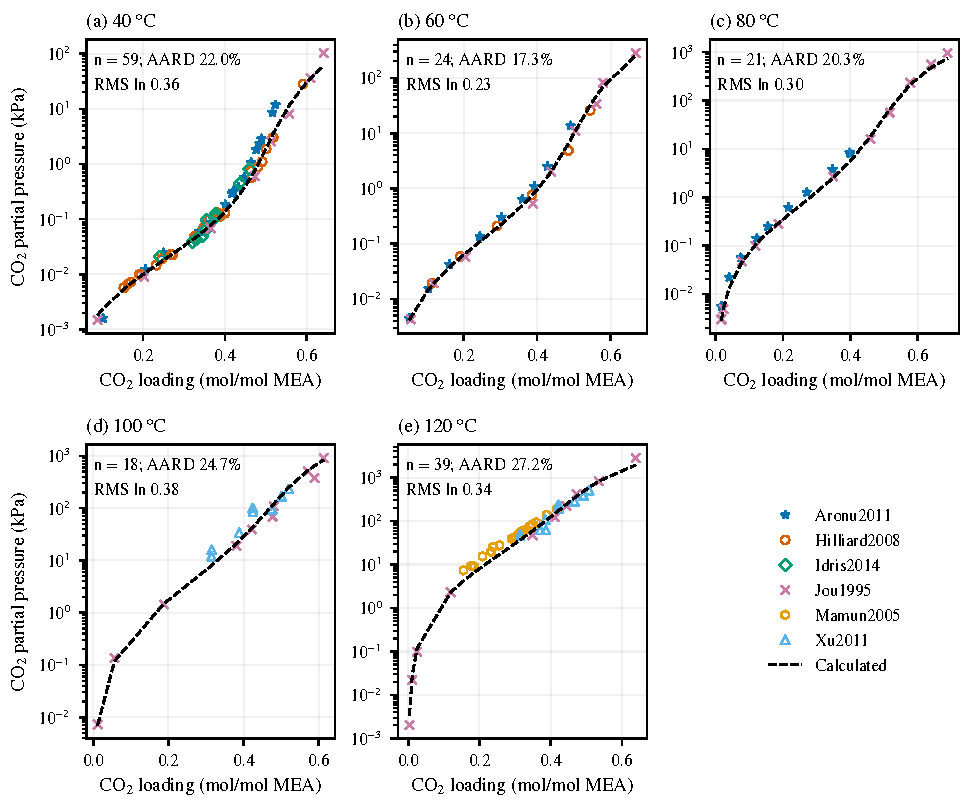
\includegraphics[width=\linewidth]{pressure.pdf}
    \caption{F1 and the source-law fit F6 agree at the fitted 40 and \SI{60}{\degreeCelsius} isotherms, but F6 underestimates the measured \COtwo partial pressures above \SI{60}{\degreeCelsius}.
    \COtwo partial pressure against loading in 30 wt\% \MEA for 159 measured pressures from six studies, grouped by nominal temperature, and for 23 Wagner et al.\ pressures near \SI{353}{\kelvin} (c) and \SI{392}{\kelvin} (e).
    Open markers are measurements; dots (F1) and crosses (F6) are calculated at each measured state and are not interpolated.
    Only the 40 and \SI{60}{\degreeCelsius} panels contain fitted pressures.
    Three Xu and Rochelle rows above \SI{393.15}{\kelvin} are not evaluated and not shown.}
    \label{fig:pressure}
\end{figure}

\begin{figure}[pos=!htb]
    \centering
    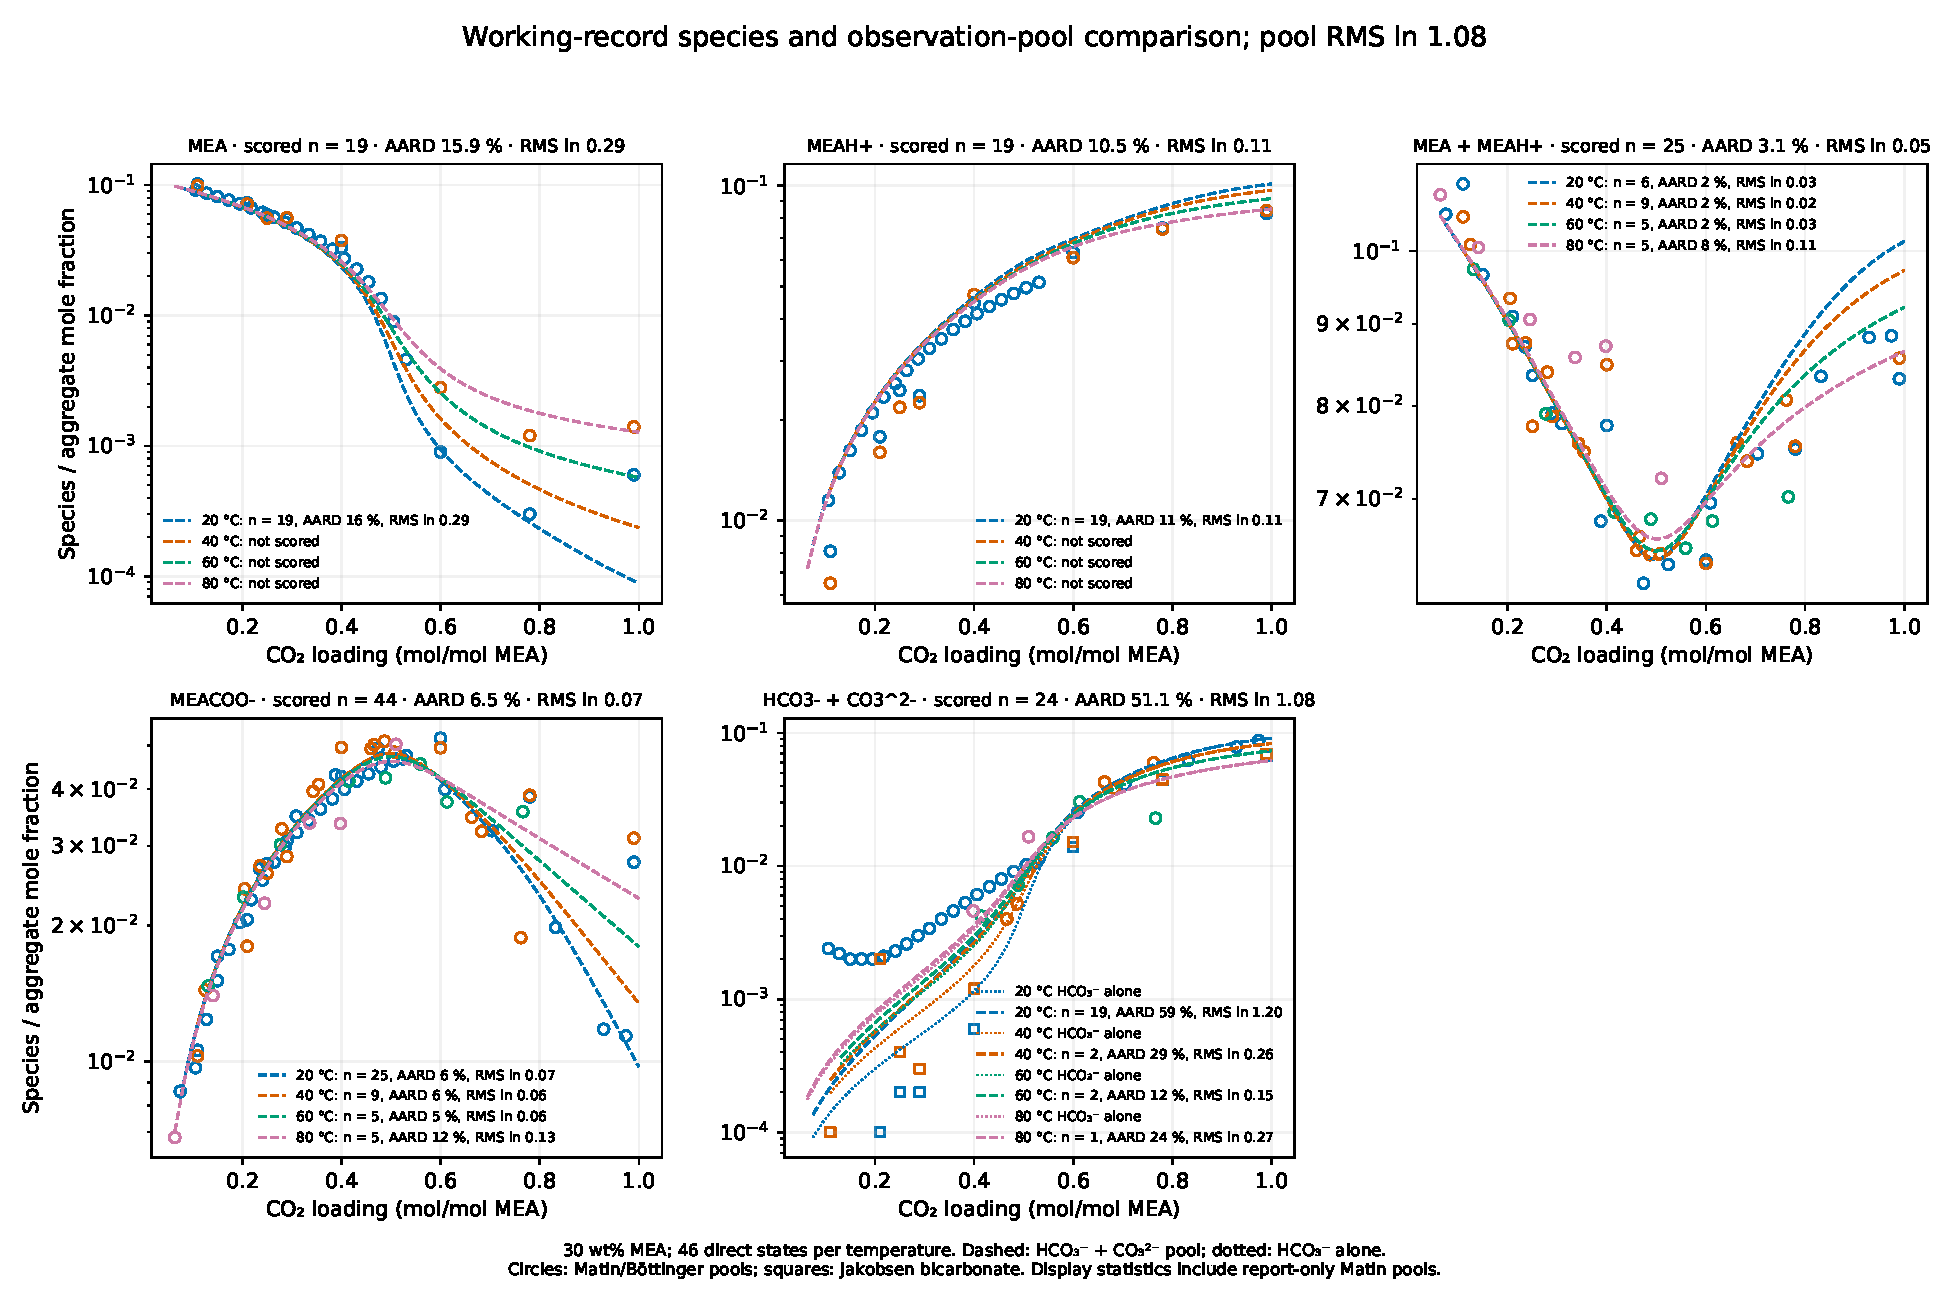
\includegraphics[width=\linewidth]{speciation.pdf}
    \caption{F1 reproduces the fitted NMR and titration species at 20--\SI{60}{\degreeCelsius}, whereas the titration bicarbonate pool, which is not fitted, lies mostly above the calculated values.
    Liquid mole fraction against loading in 30 wt\% \MEA: (a) 76 titration values of Matin et al.\ at \SI{20}{\degreeCelsius}; (b)--(e) 55 NMR values of B\"ottinger et al., where \MEA and \MEAH are observed only as a sum.
    Circles are fitted measurements, squares are measurements outside the fit, and dots are F1 calculations at each measured state, joined to their measurement by a vertical segment.
    Bicarbonate values of both sources are compared with the modeled \ce{HCO3- + CO3^2-} pool.
    Matin's measurements, labeled \SI{21}{\degreeCelsius} in the source figures, are calculated at \SI{20}{\degreeCelsius}.}
    \label{fig:speciation}
\end{figure}

% P:results-03
At F1 the \HCOthree--water coefficient lies on its upper bound of \(+0.5\), with an outward cost gradient of \(-12.63\), so the cost would decrease further if the bound were relaxed; its value is set by the bound rather than estimated from the data.
For the four interior parameters, the conditional standard errors are 0.014 for \(k_{\MEACOO,\HtwoO}\), 0.017 for \(k_{\MEAH,\HtwoO}\) and 0.027 for \(k_{\MEAH,\MEACOO}\) (\cref{tab:binary-interaction-parameters}), and the largest correlation, 0.46, links \(k_{\MEAH,\HtwoO}\) with its slope \(b\).
The slope itself is \(b=\SI{-112.6}{\kelvin}\) with a conditional standard error of \SI{119.7}{\kelvin}, so these data, which constrain temperature only through pressures at 40 and \SI{60}{\degreeCelsius} and species at 20--\SI{60}{\degreeCelsius}, do not determine it.
It is retained so that all six fits share the same five parameters.
These standard errors rest on the declared residual scales and on residuals treated as independent (\cref{sec:data-methods}), and they are indicative only.

\subsection{Born term}\label{sec:results-born-off}
% P:results-04
Refitting all five parameters without the Born term (F3), within the same bounds and from two starts, gives a fitted-pressure AARD of 53.60\,\% and a fitted-species AARD of 10.79\,\%, against 13.98 and 8.26\,\% for F1.
The cost rises from 33.03 to 96.64, and the pressure targets carry 53.17 of this increase.
Both the \HCOthree--water and the \MEAH--\MEACOO coefficients reach their bounds, \(+0.5\) and \(-1\).
The tested refits within the declared bounds therefore do not recover the agreement of the model with a Born term; this result concerns these parameters and bounds and does not show that a Born contribution is physically necessary.

% P:results-05
A decomposition of the calculated pressure locates where the refit loses agreement.
Combining \COtwo phase equilibrium with the overall carbamate reaction R2 \(-\) R4 \(-\) R5, \(\ce{CO2 + 2 MEA <=> MEAH+ + MEACOO-}\), gives at every calculated state
\begin{equation}
    \ln p_{\COtwo}=S+Q-\ln K_{x,\mathrm{OV}}+H,
    \qquad
    S=\ln\frac{x_{\MEAH}\,x_{\MEACOO}}{x_{\MEA}^{2}},
    \label{eq:pressure-decomposition}
\end{equation}
where \(S\) is the speciation sum, \(Q=\sum_i\nu_{\mathrm{OV},i}\ln\gamma_i^{*}+\ln\gamma_{\COtwo}^{*}\) is the activity sum of the overall reaction, in which the \COtwo activity coefficient cancels, \(K_{x,\mathrm{OV}}\) is the mole-fraction equilibrium constant of the overall reaction, and \(H\) collects the vapor fugacity coefficient and reference fugacity of \COtwo.
At fixed speciation, liquid nonideality changes the \COtwo pressure only through \(Q\), and each Helmholtz contribution adds its own part to \(Q\).
For F3 relative to F1, \cref{eq:pressure-decomposition} splits the change of \(\ln p_{\COtwo}\) at each fitted pressure state into \(\Delta Q\), \(\Delta S\) and \(\Delta H\); the split reproduces the pressure-cost increase of 53.17 and closes within \(10^{-6}\) at every state (Supplementary Section~S3).

\begin{figure}[pos=!htb]
    \centering
    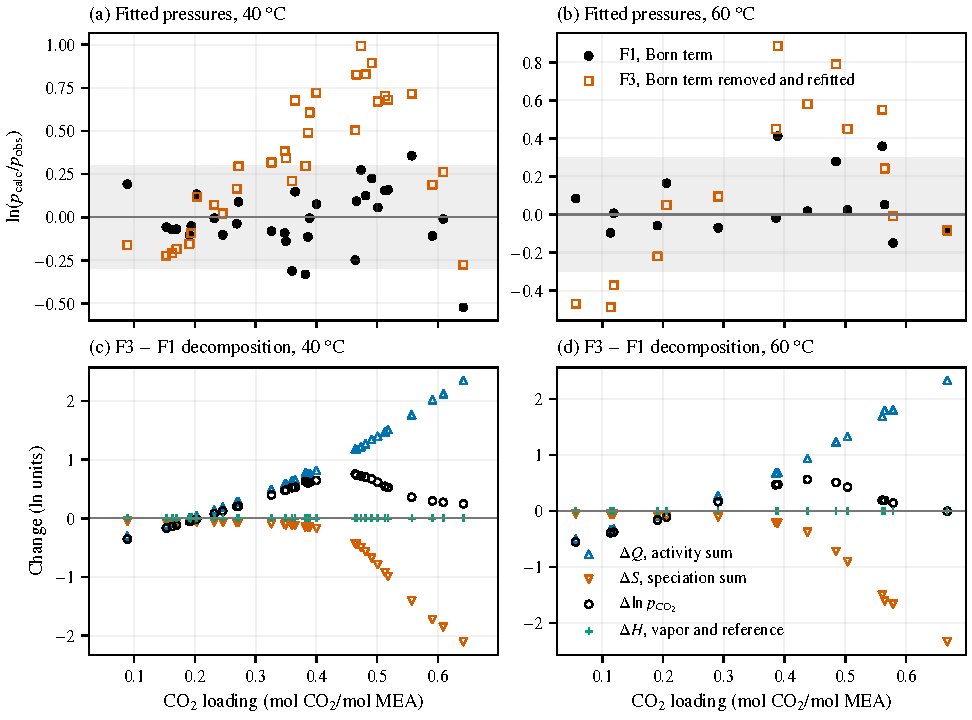
\includegraphics[width=\linewidth]{born-off-mechanism.pdf}
    \caption{Without the Born term, the refitted model F3 overestimates the fitted pressures at intermediate loadings, because the activity sum \(Q\) rises with loading faster than the speciation sum \(S\) falls.
    (a, b) \(\ln(p_{\mathrm{calc}}/p_{\mathrm{obs}})\) of the 47 fitted pressures for F1 and F3 in the nominal 40 and \SI{60}{\degreeCelsius} series; the shaded band is \(\pm0.3\), the declared pressure residual scale, not an acceptance interval.
    (c, d) Change from F1 to F3 of \(\ln p_{\COtwo}\) and of its contributions in \cref{eq:pressure-decomposition} at the same states.
    Points are calculated states at their measured temperatures and are not interpolated.}
    \label{fig:born-off}
\end{figure}

% P:results-06
Over the 47 fitted pressure states, the root-mean-square change of \(Q\), 1.09, exceeds that of \(S\), 0.82, so the refit changes the activity sum more than the speciation in aggregate (\cref{fig:born-off}).
\(\Delta Q\) rises with loading to about 2.3 at the highest loadings, where a nearly equal and opposite \(\Delta S\) cancels most of it; the net change of \(\ln p_{\COtwo}\) is largest at intermediate loadings, where F3 overestimates the measured pressures.
Two tests stated before the calculation locate the Born contribution of F1.
First, the Born part of the activity-coefficient sum \(\sum_i\nu_{\mathrm{OV},i}\ln\gamma_i^{*}\) of the overall reaction is negative, with a median of \(-0.91\) over the 32 fitted states at \SI{40}{\degreeCelsius}, and at the median-loading state its permittivity part, \(-0.29\), is less than half of the total, \(-0.88\); the hypothesis that the Born term raises this sum through the lower permittivity of \MEA--water is therefore rejected.
Second, the ion-concentration part of the Born contribution to \(Q\), defined as the Born contribution minus its value at the ion-free composition of the same state, falls steadily with loading: its Spearman correlation with loading is \(-0.997\) at \SI{40}{\degreeCelsius} and \(-0.996\) at \SI{60}{\degreeCelsius}, and its mean over the highest-loading third of the states is \(-1.76\) and \(-1.75\).
The non-Born activity changes of the refit offset the removed Born contribution fully or more in the lowest-loading third, with mean offset fractions of 1.00 and 1.58 at 40 and \SI{60}{\degreeCelsius}, but hardly at all in the highest-loading third, with 0.08 and \(-0.01\).
Within this model, the Born term therefore supplies a loading-dependent lowering of the activity sum that the five refitted interactions reproduce at low loading but not at high loading.
These are attributions within the calibrated model at its fitted states, under stated conventions for splitting the Born term; they are not measurements of single-ion activity coefficients.

\subsection{Born form and fitted observation set}\label{sec:results-born}
% P:results-07
The SSM+DS (F1) and original Born (F2) forms were fitted with the same parameters, bounds, weights, reaction constants and ion inputs, and they calibrate the data comparably.
With Matin's 18 pool targets not fitted, SSM+DS has the lower cost, 33.03 against 34.14, and the lower fitted-pressure AARD, 13.98 against 17.36\,\%, whereas original Born has the slightly lower fitted-species AARD, 8.16 against 8.26\,\% (\cref{tab:residual-summary}).
In F2 the \MEAH--\MEACOO coefficient also lies on its lower bound of \(-1\).
These are local cost comparisons, not statistical tests.

% P:results-08
Matin et al.\ obtained bicarbonate from a titration that assigns carbonate to bicarbonate, and they report bicarbonate above the NMR values of Jakobsen et al., whereas their free amine, protonated amine and carbamate agree more closely (Fig.~2, p.~6616; Fig.~3 and discussion, p.~6617)~\cite{matinFacileMethodDetermination2012,Jakobsen2005}.
On that basis the 18 Matin pool targets are not fitted in F1 and F2.
F1 lies below them, with an AARD of 59.59\,\% and a mean \(\ln(x_{\mathrm{calc}}/x_{\mathrm{obs}})\) of \(-1.06\), and F2 gives 34.99\,\%.

\begin{figure}[pos=!htb]
    \centering
    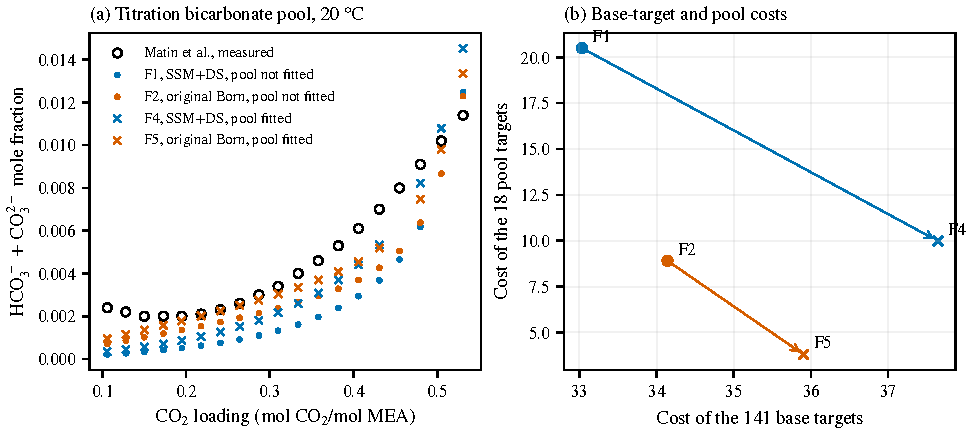
\includegraphics[width=\linewidth]{pool-effect.pdf}
    \caption{Fitting Matin's titration bicarbonate pool reverses the Born-form ranking.
    (a) \ce{HCO3- + CO3^2-} mole fraction at \SI{20}{\degreeCelsius}: Matin et al.\ measurements and the values calculated by F1 and F2, which do not fit the pool, and by F4 and F5, which fit it; the Matin state at loading 0.455 is outside both target sets.
    (b) Cost of the 141 base targets against the cost of the 18 pool targets; arrows join each Born form's fit without and with the pool.}
    \label{fig:pool-effect}
\end{figure}

% P:results-09
Adding the 18 pool targets to the objective reverses the order of the two forms (\cref{fig:pool-effect}): original Born then has the lower cost, 39.70 against 47.63 for SSM+DS.
Fitting the pool lowers its AARD to 42.57\,\% for SSM+DS (F4) and 19.56\,\% for original Born (F5), while the cost of the 141 base targets rises from 33.03 to 37.64 and from 34.14 to 35.91.
Original Born therefore moves toward the titration bicarbonate at a smaller cost to the other targets.
For these data, the pressure and speciation fits give no preference between the two Born formulations that is independent of the fitted observations, and independent solvation or activity data could help choose between them.
The residual signs do not establish which bicarbonate measurement is correct.

\subsection{Temperature and concentration outside the fit}\label{sec:results-80c}
% P:results-10
The R2 and R5 reaction shifts and the \COtwo dispersion energy of F1 and F2 were estimated with data that included \SI{80}{\degreeCelsius} (\cref{sec:data-methods}), so the comparisons at \SI{80}{\degreeCelsius} and above test conditions outside the five-parameter fit but are not independent temperature predictions.
On the 21 measured pressures at \SI{80}{\degreeCelsius}, F1 gives an AARD of 19.58\,\% with a mean \(\ln(p_{\mathrm{calc}}/p_{\mathrm{obs}})\) of \(-0.170\); the 11 Jou et al.\ measurements alone give 9.57\,\%.
For the 11 B\"ottinger species at \SI{80}{\degreeCelsius}, measured in a 31 wt\% solution, F1 gives 12.05\,\% and F2 8.08\,\%.
The 23 Wagner et al.\ pressures entered no fit or parameter selection; F1 gives 22.50\,\% with a mean \(\ln(p_{\mathrm{calc}}/p_{\mathrm{obs}})\) of \(-0.257\) on the 11 rows near \SI{353}{\kelvin} and 22.27\,\% with \(-0.265\) on the 12 rows near \SI{392}{\kelvin}, so it underestimates these pressures on average.
At 100--\SI{120}{\degreeCelsius}, the 54 evaluated pressures give 27.24\,\%.
These temperatures lie above the \SI{323.15}{\kelvin} upper limit of the R4 and R5 source correlations, so these values are extrapolations.
F2 gives similar values in each of these pressure groups (\cref{tab:residual-summary}).

% P:results-11
On the 105 measured pressures at 40--\SI{80}{\degreeCelsius}, F1 gives an AARD of 20.35\,\%.
This group combines fitted targets with rows outside the fit, so it measures pooled agreement, not accuracy outside the fit.
By source, the AARDs are 31.76\,\% for Aronu et al.\ (36 rows), 11.40\,\% for Hilliard (31 rows), 15.59\,\% for Jou et al.\ (28 rows) and 20.32\,\% for Idris et al.\ (10 rows)~\cite{Aronu2011,Hilliard2008,Jou1995,idrisSpeciationMEACO2Adducts2014}.
The mean \(\ln(p_{\mathrm{calc}}/p_{\mathrm{obs}})\) is \(-0.381\) for the Aronu rows and \(-0.136\) for all 105, so the pooled value is dominated by underestimation of the Aronu measurements.

% P:results-12
Applied unchanged at other amine concentrations, F1 gives AARDs of 76.71\,\% on 33 Aronu et al.\ pressures at 15 wt\% \MEA and 46.29\,\% on 37 at 45 wt\%, with mean \(\ln(p_{\mathrm{calc}}/p_{\mathrm{obs}})\) of \(+0.458\) and \(-0.522\), so the error changes sign with amine concentration and the parameters are calibrated for 30 wt\% \MEA.
Over nine Jakobsen NMR points at 20 and \SI{40}{\degreeCelsius}, the calculated carbonate share of dissolved carbon is 0.41--1.34 times the observed share for F1 and 1.19--3.21 times for F2~\cite{Jakobsen2005}.
The excluded point at \SI{40}{\degreeCelsius} and loading 0.21 has an observed share of 0.119, against 0.010--0.019 at the other four \SI{40}{\degreeCelsius} loadings, and the source dilution and loading definitions are unresolved; all ten comparisons are listed in the Supplementary Material.

\subsection{Source reaction laws}\label{sec:results-source-laws}
% P:results-13
F6 uses a different temperature description with the same 141 targets: R2 and R5 follow their source correlations, the \COtwo dispersion energy is the published \SI{169.21}{\kelvin}, and the five interaction parameters are refitted.
It fits the data at or below \SI{60}{\degreeCelsius} as well as F1, with a cost of 33.06 against 33.03, but represents higher temperatures worse (\cref{fig:pressure}).
On the 21 measured pressures at \SI{80}{\degreeCelsius} it gives 28.91\,\% against 19.58\,\%, on the Wagner rows near \SI{353}{\kelvin} 51.60\,\% against 22.50\,\%, and on the 54 evaluated pressures at 100--\SI{120}{\degreeCelsius} 51.05\,\% against 27.24\,\%, with a mean \(\ln(p_{\mathrm{calc}}/p_{\mathrm{obs}})\) of \(-0.731\) on the last group, so its calculated pressures are too low.
At 15 wt\% \MEA, F6 gives 31.12\,\% against 76.71\,\% for F1; at 45 wt\% it gives 55.18\,\% against 46.29\,\%.

% P:results-14
F6 changes the reaction laws, the \COtwo dispersion energy and the refitted interactions together, so the difference from F1 does not isolate the effect of the reaction laws.
Both fits use their reaction correlations over the same declared domain, 293.15--\SI{393.15}{\kelvin}, which extends beyond the source ranges; the R4 source correlation, for example, ends at \SI{323.15}{\kelvin}.
The comparison therefore assesses extrapolated model behavior.
Data at or below \SI{60}{\degreeCelsius} do not distinguish between the two temperature descriptions, and the higher-temperature agreement of F1 rests on shifts estimated with \SI{80}{\degreeCelsius} data.
For modelers, the temperature response of this model must come from data that carry it directly, such as heat of absorption or equilibrium measurements above \SI{60}{\degreeCelsius}.

\subsection{Comparison with published models}\label{sec:results-literature}
% P:results-15
Like the electrolyte NRTL model of Zhang et al., which was fitted to \COtwo solubility, heat of absorption, heat capacity and NMR speciation~\cite{Zhang2011}, and unlike that of Akula et al., which left NMR speciation outside its fit~\cite{Akula2023a}, the present model fits speciation together with pressure, so the residuals of its 94 fitted species targets are calibration results (\cref{tab:literature-model-comparison}).
Unlike the ePC-SAFT models of MDEA~\cite{Uyan2015,Wangler2018,Bulow2021a}, it fits ion interactions to the loaded ternary mixture, including the \MEAH--\MEACOO interaction, which exists only in loaded solution.
Published pressure deviations for 30 wt\% \MEA cover different row sets and temperature ranges, so no accuracy ranking against those models is claimed.

\subsection{Scope and limitations}\label{sec:results-limits}
% P:results-16
F1 describes \COtwo partial pressure in 30 wt\% \MEA, fitted at 40 and \SI{60}{\degreeCelsius}, and liquid speciation, fitted at 20--\SI{60}{\degreeCelsius}; its comparisons at 80--\SI{120}{\degreeCelsius} rest partly on reaction shifts estimated with \SI{80}{\degreeCelsius} data.
Its ion parameters are effective values: the \MEAH and \MEACOO parameters were fitted to speciation data, the \HCOthree--water coefficient lies on its bound, and the \MEAH--water slope is not determined.
The conditional standard errors treat residuals as independent and exclude the uncertainty of the fixed inputs.
The Matin values are a transcription not checked against the source's supporting tables.

% P:results-17
Liquid density is not fitted.
At an assumed pressure of \SI{101325}{\pascal}, which the source does not report, F1 overpredicts the four loaded densities of Amundsen et al.\ at 50 and \SI{70}{\degreeCelsius} and loadings 0.3 and 0.4~mol \COtwo/mol \MEA, on a \COtwo-free 30 wt\% \MEA solvent basis, by 13.0--17.8\,\%~\cite[Table~3, p.~3097]{Amundsen2009}.
The source gives a general uncertainty estimate of \(\pm\SI{0.002}{\gram\per\cubic\centi\metre}\) for loaded solutions but excludes the highest temperatures and loadings from it~\cite[pp.~3099--3100]{Amundsen2009}, so these deviations are not weighted by uncertainty.
Heat capacity and heat of absorption were not evaluated for F1.
The parameter set is therefore a phase- and speciation-equilibrium model; absorber and stripper calculations would require density and caloric qualification first.

\section{Conclusions}\label{sec:conclusion}
% P:conclusion-01
Electrolyte PC-SAFT with Debye--H\"uckel and Born contributions and explicit carbamate chemistry describes \COtwo partial pressure and liquid speciation in 30 wt\% aqueous \MEA with one set of liquid-phase parameters.
Fitted through five binary interaction parameters to 47 \COtwo pressures at 40 and \SI{60}{\degreeCelsius} and 94 species measurements at 20--\SI{60}{\degreeCelsius}, the nine-species model reaches AARDs of 13.81 and 7.89\,\%.
On Wagner et al.\ pressures near 80 and \SI{119}{\degreeCelsius} (353 and \SI{392}{\kelvin}), which entered no fitting or selection step, it gives 23.11 and 16.23\,\%; the other data at 80--\SI{120}{\degreeCelsius} informed fixed reaction shifts and are not independent temperature tests.
This extends the ePC-SAFT treatment of reactive MDEA to a carbamate-forming primary amine.

% P:conclusion-02
Within the tested model, bounds, objective and two starts, refitting without the Born term raises fitted-pressure AARD from 13.81 to 80.25\,\%.
This establishes neither physical necessity nor a mechanism.
SSM+DS has the lower total cost both without and with the titration bicarbonate pool; fitting the pool does not reverse the ordering.

% P:conclusion-03
Heat measurements give the \MEAH--water reciprocal-temperature slope \(b=\SI{107.96}{\kelvin}\) with conditional standard error \SI{22.93}{\kelvin}, while the \HCOthree--water coefficient remains on its bound.
The uncertainty conditions on fixed inputs, active bounds and declared residual scales.
The source-law refit has a similar pressure/species subtotal but poorer heat agreement and a canonical 100--\SI{120}{\degreeCelsius} pressure AARD of 54.98\,\%.
These comparisons constrain this parameterization without uniquely locating its limitation in reaction chemistry.

% P:conclusion-04
Applied unchanged at 15 and 45 wt\% \MEA, the selected parameter set gives pressure AARDs of 105.54 and 56.32\,\%.
A separate density-only translation gives deviations of \(-0.15\) to \(+0.25\)\,\% over its four calibration states; these are calibration results rather than independent density predictions.
Density transfer, solution heat capacity and wider calorimetric agreement remain limitations before absorber or stripper use.
\section*{Data and Code Availability}
% P:availability-01
\textit{Data availability statement pending the public deposit or immutable manuscript tag.}
The Supplementary Material lists the calculation files and software identities used by this draft.

\section*{Funding}
% P:availability-02
This research received no specific grant from funding agencies in the public, commercial, or not-for-profit sectors.

\section*{Declaration of Competing Interest}
% P:availability-03
The author declares no known competing financial interests or personal relationships that could have appeared to influence the work reported in this paper.

\section*{CRediT Author Statement}
% P:availability-04
Tanner W. Polley: Conceptualization, methodology, software, validation, formal analysis, investigation, data curation, writing--original draft, writing--review and editing, and visualization.

\section*{Declaration of Generative AI and AI-Assisted Technologies}
% P:availability-05
During preparation of this manuscript, OpenAI Codex and Claude (Anthropic) were used to draft and revise manuscript text, check computational consistency, and assist with bibliography checking and correction.
The author reviewed and edited the content and takes responsibility for the final manuscript.


\clearpage
\bibliographystyle{styles/model1-num-names}
\bibliography{references}

\clearpage
\phantomsection
\noindent\begin{minipage}{\linewidth}
    \centering
    \captionsetup{hypcap=false}
    \captionof{table}{Symbols used in this manuscript.}
    \label{tab:nomenclature}
    \small
    \begin{tabularx}{\linewidth}{lX}
        \toprule
        Symbol & Definition \\
        \midrule
        \(\alpha\) & \COtwo loading (mol \COtwo per mol total amine) \\
        \(T\), \(T_{\mathrm{ref}}\) & Temperature; reference temperature of \cref{eq:kij-temperature}, \SI{313.15}{\kelvin} \\
        \(P\), \(p_{\COtwo}\) & Bubble pressure; \COtwo partial pressure, \(y_{\COtwo}P\) \\
        \(x_i\), \(y_i\) & Liquid and vapor mole fraction of true species \(i\) \\
        \(z_i\), \(M_i\) & Charge number and molar mass of species \(i\) \\
        \(a^{\mathrm{res}}\) & Reduced residual Helmholtz energy and its contributions (hc, disp, assoc, DH, Born) \\
        \(m_i\), \(\sigma_i\), \(u_i/k_{\mathrm{B}}\) & Segment number, segment diameter and dispersion energy \\
        \(k_{ij}\), \(b\) & Binary dispersion interaction parameter; its reciprocal-temperature slope (K) \\
        \(\kappa^{AB}\), \(\epsilon^{AB}/k_{\mathrm{B}}\) & Association volume and association energy \\
        \(d_i^{\mathrm{Born}}\), \(D_i\) & Born diameter; outer diameter of the first solvation shell \\
        \(f_k\), \(f_{\mathrm{mix}}\) & Solvation factor of component \(k\); its mole-fraction average \\
        \(c_{\mathrm{shell}}\), \(c_{\mathrm{dielectric}}\) & Born-form coefficients: (1,1) for SSM+DS, (0,0) for original Born \\
        \(\varepsilon_{\mathrm{bulk}}\), \(\varepsilon_{\mathrm{ion}}\), \(\varepsilon_s\) & Relative permittivity of the solution, of the region next to an ion, and of solvent \(s\) \\
        \(\nu_{ri}\), \(K_r\), \(a_i\) & Stoichiometric coefficient, equilibrium constant of reaction \(r\), activity of species \(i\) \\
        \(A_r\), \(B_r\), \(C_r\), \(D_r\), \(\Delta_r\) & Coefficients of \(\ln K_r(T)\); offset to the aqueous-molality basis \\
        \(m^{\circ}\) & Standard molality, \SI{1}{\mole\per\kilo\gram} \\
        \(r_{P,j}\), \(r_{x,j}\), \(C\) & Weighted pressure and species residuals; fitting cost \(\tfrac12\sum_jr_j^2\) \\
        AARD & Average absolute relative deviation, \cref{eq:aard} \\
        \(\gamma_i^{*}\) & Activity coefficient of species \(i\) on the standard state of its source constant \\
        F1--F6 & The six fits of \cref{sec:data-methods}; F1 is the selected parameter set \\
        \bottomrule
    \end{tabularx}
\end{minipage}\par


\end{document}

